\documentclass[12pt, titlepage]{article}
\usepackage{float}
\usepackage{booktabs}
\usepackage{tabularx}
\usepackage{hyperref}
\usepackage{indentfirst}
\usepackage{enumerate}
\usepackage{graphicx}
\usepackage{cite}

\hypersetup{
    colorlinks,
    citecolor=black,
    filecolor=black,
    linkcolor=red,
    urlcolor=blue
}

\title{SFWRENG 3XA3: Software Requirements Specification\\Rummy For Dummies}

\author{Lab 2 Group 7, Rummy For Dummies
		\\ Joy Xiao, xiaoz18
		\\ Benson Hall, hallb8
		\\ Smita Singh, sings59
}

\date{\today}

\begin{document}

\maketitle

\pagenumbering{roman}
\tableofcontents
\listoftables
\listoffigures

\begin{table}[bp]
\caption{\bf Revision History}
\begin{tabularx}{\textwidth}{p{3cm}p{2cm}X}
\toprule {\bf Date} & {\bf Version} & {\bf Notes}\\
\midrule
Feb. 12, 2021 & 1.0 & Revision 0 of SRS document.\\
\bottomrule
\end{tabularx}
\end{table}

\newpage

\pagenumbering{arabic}

This document describes the requirements for Rummy for Dummies.
This document will be used as a reference point for all future documentation and development. This requirement specification document follows the Volere template \cite{volere}.

\section{Project Drivers}

\subsection{The Purpose of the Project}
The purpose of this project will be to recreate the open-source version of Gin Rummy. Gin Rummy is a popular, multi-player game, liked by many people. This implementation is targeted towards individuals seeking to entertain themselves while remaining in their homes during lockdown. The project will convert a conventionally multiplayer game, so that it can be played alone with a computer opponent. The game will be easy to use and play, and be more visual than the open-source version.

\subsection{The Stakeholders}

\subsubsection{The Client}
The clients of the project will be the teaching assistants of SFWRENG 3XA3 and Dr. Bokhari. They will provide insight and assistance throughout the development of this project.

\subsubsection{The Customers}
The customers of the project will be card game enthusiasts, and individuals of all ages looking to play a game of Gin Rummy or variants of the game.

\subsubsection{Other Stakeholders}
The other stakeholders include the developers, who will be working to implement a improved version of the open-source project.
\subsection{Mandated Constraints}

\subsubsection{Solution Constraints}
\noindent Description: The project shall be written in Java and unit tested using JUnit.

\noindent Rationale: The developers are already familiar with using Java and JUnit, making this an ideal choice.

\noindent Fit Criterion: The source code will be written entirely in Java. \\

\noindent Description: The game shall be played through the CLI.

\noindent Rationale: It ensures that the game is simple for users to play and has a minimalist interface, which uses less resources.

\noindent Fit Criterion: The project will have no GUI, and will use ASCII characters to represent cards to create the visual experience for users on the CLI. \\

\noindent Description: The program will be used on operating systems such as Windows, MacOS and Linux.

Rationale: These operating systems can run the project without any additional installations.

Fit Criterion: The project will be made to compile and execute on the above stated operating systems. \\

\subsubsection{Implementation Environment of the Current System}


\subsubsection{Partner or Collaborative Applications}
This implementation does not have any partner or collaborative applications. It relies solely on the operating system to run a Java application.

\subsubsection{Off-the-Shelf Software}
There is no current off-the-shelf software that the developers will use within the implementation. 

\subsubsection{Anticipated Workplace Environment}
The anticipated workplace environment is the user's home. However, the product can run on most desktop or laptop computers anywhere. There is no need for an internet connection, and the game can be played locally on the user's machine.

\subsubsection{Schedule Constraints}
The project must be completed by the week of April 5th, 2021. This is when the final demonstration will take place.

\subsubsection{Budget Constraints}
The budget is \$0 because there is no monetary funding. Creating this project should have no monetary cost, because there will be no costly resources used.

\subsubsection{Enterprise Constraints}
The game is free to download and play on the CLI for any user.

\subsection{Naming Conventions and Terminology}
\begin{table}[H]
\caption{Naming Conventions and Terminology}
    \centering
    \begin{tabular}{ |p{5cm}|p{7.5cm}| }
    \hline
    \textbf{Term} & \textbf{Definition} \\
    \hline
    CLI & Command Line Interface \\
    \hline
    JRE & Java Runtime Environment \\
    \hline
    GUI & Graphical User Interface \\
    \hline
    Stock Pile & Remaining cards in the deck after dealing \\
    \hline
    Discard Pile & Cards that were discarded by the players \\
    \hline
    Deadwood Cards & Cards that are not part of a meld \\
    \hline
    Meld & Cards that form a valid sequence or have a common value \\
    \hline
    \end{tabular}
\end{table}

\subsection{Relevant Facts and Assumptions}

The project will implement a specific variant of Gin-Rummy. \cite{ginRuleSet}

\section{Functional Requirements}
\subsection{The Scope of the Work and the Product}
Currently, launching the original source project and play a game of Gin Rummy requires the code to be compiled and built before operation. As the code is built in Go, it requires an installation of Go to compile and execute. \cite{ogSource}

As a command line and JRE generally come with a majority of desktop computers, the goal is to re-create Gin Rummy in Java for general use.
\subsubsection{The Context of the Work}
This project is to be developed for the SFWRENG 3XA3 course. It is developed for the professor of the course, Dr. Asghar Bokhari, and the teaching assistant assigned to our team, Mehdi Jafarizadeh.

Prior to development of the implementation, several documents will be created to efficiently establish the logistics of the project. These documents include:
\begin{itemize}
    \item Test Plan
    \item Development Plan
    \item Module Guide
    \item Module Interface Specifications
\end{itemize}

The plan is to re-implement Gin Rummy in Java and to make it more accessible to the general public. The project will be developed such that it can be easily compiled and run in the command line.

\subsubsection{Work Partitioning}
\begin{table}[H]
\caption{Work Partitioning Events}
    \centering
    \begin{tabular}{|c|p{3.5cm}|c|p{3.5cm}|}
    \hline
    \textbf{Event Number} & \centering\textbf{Event Name} & \textbf{Input} & \textbf{Output} \\
    \hline
    1 & Starting the Game & Keyboard & New Game \\
    \hline
    2 & Reading the Rules & Keyboard & Rules \\
    \hline
    3 & Draw A Card from the Stock Pile & Keyboard & Request to Discard Card \\
    \hline
    4 & Discard A Card to Discard Pile & Keyboard & Manipulated Hand \\
    \hline
    5 & Draw A Card from Discard Pile & Keyboard & Request to Discard Card \\
    \hline
    6 & Check All Melds in Hand & Keyboard & Current Melds in Player's Hand \\
    \hline
    7 & Check the Current Score of Hand & Keyboard & Hand Score \\
    \hline
    8 & Player knocks & Keyboard & Calculated Score \& New Round \\
    \hline
    \end{tabular}
\end{table}

\begin{table}[H]
\caption{Work Partitioning Summaries}
    \centering
    \begin{tabular}{|c|p{10cm}|}
    \hline
    \textbf{Event Number} & \textbf{Summary} \\
    \hline
    1 & The user, through the keyboard input, decides to start a new game of Gin Rummy. \\
    \hline
    2 & The user, through keyboard input, chooses to read the rules of Gin Rummy. \\
    \hline
    3 & If the user chooses to draw a card from the stock pile, they must discard a card from their hand after the card is added to their hand. \\
    \hline
    4 & The user selects a card to add to the discard pile through keyboard input. \\
    \hline
    5 & If the user chooses to draw a card from the discard pile, they must discard a card from their hand after adding the card to their hand. \\
    \hline
    6 & If the user wishes to see all their melds, a list of all possible melds are displayed. \\
    \hline
    7 & If the user wishes to see their current score, the score will be calculated from the deadwood cards currently in their hand. \\
    \hline
    8 & If the user wishes to knock and has a score less than or equal to 10, the round ends and points are calculated based on deadwood score of both sides. \\
    \hline
    \end{tabular}
\end{table}
\subsubsection{Individual Product Use Cases}

\begin{figure}[H]
    \centering
    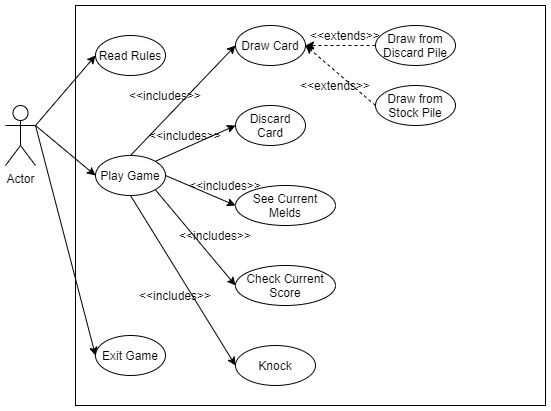
\includegraphics[scale=0.5]{3xa3UseCase.jpg}
    \caption{Use Case Diagram}
    \label{fig:useCase}
\end{figure}

\subsection{Functional Requirements}
\textbf{Business Event 1:} The user wants to start a new game.
\begin{itemize}
    \item FR1. The system shall ask the user to input their name.
    \item FR2. The system shall display a random set of cards as the users card hand, and it shall display the top card on the discard pile.
    \item FR3. The system shall display the set of options the user can take.
\end{itemize}

\textbf{Business Event 2}: The user wants to draw a card from the stock pile.
\begin{itemize}
    \item FR4. The system shall add the top card of the stock pile to the user's hand.
    \item FR5. The system shall display the new card to the user through the CLI.
    \item FR6. The system shall prompt the user to discard one of the cards in their hand.
\end{itemize}

\textbf{Business Event 3}: The user wants to pick up a card from the discard pile.
\begin{itemize}
    \item FR7. The system shall add the top card on the discard pile to the user's hand.
    \item FR8. The system shall display the new card to the user through the CLI.
    \item FR9. The system shall prompt the user to discard one of the cards in their hand.
\end{itemize}

\textbf{Business Event 4}: The user wants to check for melds. 
\begin{itemize}
    \item FR10. The system shall show the user any melds that can be created from the user's hands.
\end{itemize}

\textbf{Business Event 5}: The user wants to check total points of the hand.
\begin{itemize}
    \item FR11. The system shall calculate and display the user's points.
\end{itemize}

\textbf{Business Event 6}: The user wants to discard a card.
\begin{itemize}
    \item FR12. The system shall prompt the user to input which card the user wants to discard.
    \item FR13. The system shall discard the chosen card if valid and display the new card hand.
    \item FR14. The system shall place the card on top of the discard pile faced up.
    \item FR15. The system shall make a move on behalf of the computer agent.
\end{itemize}

\textbf{Business Event 7}: The user wants to knock.
\begin{itemize}
    \item FR16. The system checks if the user has less than 10 deadwood points.
    \item FR17. If the user has 10 or fewer deadwood points, then the system shall end the round. 
    \item FR18. The system will calculate the difference in deadwood points between the user and AI and determine the winner.
    \item FR19. The system will award the points to the winner.
    \item FR20. The system will prompt the player if they want to play a new round.
\end{itemize}

\textbf{Business Event 8}: The user wants to exit the game.
\begin{itemize}
    \item FR21. The system shall terminate the game and game data will not be saved.
\end{itemize}

\section{Non-Functional Requirements}

\subsection{Look and Feel Requirements}
\begin{enumerate}[{LF}.1]
    \item The system shall have a simplistic look.
\end{enumerate}

\subsection{Usability and Humanity Requirements}
\begin{enumerate}[{UH}.1]
    \item The system shall be easy to play for users of any age.
    \item The system shall be easy to run for users of any age.
\end{enumerate}

\subsection{Performance Requirements}
\begin{enumerate}[{P}.1]
    \item The system shall respond to valid user interactions within 0.5 seconds.
    \item The system shall adhere to rules of the game Rummy.
\end{enumerate}

\subsection{Operational and Environmental Requirements}
\begin{enumerate}[{OE}.1]
    \item The system shall be able to be operated on Windows, Linux, and MacOS operating systems.
\end{enumerate}

\subsection{Maintainability and Support Requirements}
\begin{enumerate}[{MS}.1]
    \item The system shall be clearly documented and commented for ease of maintainability.
    \item The system shall be as modularized as possible.
\end{enumerate}

\subsection{Security Requirements}
N/A

\subsection{Cultural Requirements}
\begin{enumerate}[{C}.1]
    \item The system shall not have any offensive images or text.
    \item The language of the system shall be in English.
\end{enumerate}

\subsection{Legal Requirements}
\begin{enumerate}[{L}.1]
    \item This system shall adhere to the same copyright properties as the original project: MIT License.
\end{enumerate}

\subsection{Health and Safety Requirements}
There are no health and safety concerns for this project. It does not store user data and the game will not post a health concern to the user.

\section{Project Issues}
% this pertains to our project
\subsection{Open Issues}
The following issues may be encountered during development of the project:
\begin{itemize}
    \item Implementation of the computer opponent.
    \item Graphically representing playing cards in the CLI.
\end{itemize}

\subsection{Off-the-Shelf Solutions}
There are existing products on the app store that implement the game of Gin-Rummy. 

\subsection{New Problems}
One of the limitations of attempting to trace source code implementation for the computer opponent is that Go is not an object-oriented language, so it will be difficult to imitate some of the source code in Java.

Our project is played through the CLI and the user will download the files to play the game. This is a problem, as people may find it difficult to run even with sufficient documentation. 

\subsection{Tasks}
The Gantt Chart for the project will be followed for task milestones. There will be two development phases: Revision 0 and Revision 1 of the project. Revision 1 will go through documents in Revision 0 and make updates to be consistent with the final product.

\begin{table}[H]
\caption{Task due dates}
    \centering
    \begin{tabular}{ |p{7.5cm}|p{4.5cm}| }
    \hline
    \textbf{Task} & \textbf{Due Date} \\
    \hline
    Proof of Concept Demonstration & February 22, 2021 \\
    \hline
    Test Plan Revision 0 & March 5, 2021 \\
    \hline
    Design and Document Revision 0 & March 18, 2021 \\
    \hline
    Revision 0 Demonstration & March 22, 2021 \\
    \hline
    Final Demonstration & April 5, 2021 \\
    \hline
    Final Documentation & April 12, 2021 \\
    \hline
    \end{tabular}
\end{table}

\subsection{Migration to the New Product}
Not applicable.

\subsection{Risks}
There are several risks associated with the development of this project:
\begin{itemize}
\item Project size is too large
\item Difficulty testing the computer opponent 
\item Bad programming practices (i.e., modules have unclear purposes)
\end{itemize}

\subsection{Costs}
There will be no costs for this project. All resources used are free. The amount of effort spent on this product is around 6 hours a week per team member. 

\subsection{User Documentation and Training}
The README.md file in the Gitlab repository will clearly document the setup of the game and its instructions.

\subsection{Waiting Room}
Not applicable.

\subsection{Ideas for Solutions}
A solution to the issue is to trace the original project and see how it is implemented there. We may need further investigation through online resources. 

A solution to representing playing cards is to use ASCII art.

\bibliography{srs}
\bibliographystyle{unsrt}

\newpage

\section{Appendix}
\subsection{Symbolic Parameters}
\begin{itemize}
    \item TOTAL\_CARDS = 52
    \item RANK = \{A, 2, 3, 4, 5, 6, 7, 8, 9, 10, J, Q, K\}
    \item SUIT = \{HEARTS, CLUBS, DIAMONDS, SPADES\}
\end{itemize}

\end{document}